%% Draft settings
\documentclass[10pt]{article}
\usepackage{amsmath}
\usepackage{amssymb}
\usepackage{graphicx}
\usepackage{subfigure}
\usepackage{color}
 \usepackage{lineno}
\usepackage{simplemargins}
\usepackage{natbib}

% \linenumbers*[1]
 \usepackage[T1]{fontenc} % For citing barki{\dj}ija
\setkeys{Gin}{draft=false}


% Margins
\setleftmargin{1in}
\setrightmargin{1in}
\setbottommargin{1in}
\settopmargin{1in}
 
% My Commands
%\input{tensor_book_shrtcts.tex}
\newcommand{\comment}[1]{\textcolor{blue}{[{#1}]}}


%%Nadir's Shortcuts
\newcommand{\beqn}{\begin{equation}}
\newcommand{\eeqn}{\end{equation}}
\newcommand{\beqa}{\begin{eqnarray}}
\newcommand{\eeqa}{\end{eqnarray}}
\newcommand{\beqanonum}{\begin{eqnarray*}}
\newcommand{\eeqanonum}{\end{eqnarray*}}
\newcommand{\beqnonum}{\begin{equation*}}
\newcommand{\eeqnonum}{\end{equation*}}
\newcommand{\jump}{\vspace{0.5cm}}
\newcommand{\bbf}{\begin{bf}}
\newcommand{\ebf}{\end{bf}}
\newcommand{\eqnref}[1]{(\ref{#1})}
\newcommand{\defn}[1]{\begin{bf}\emph{#1}\end{bf}}
\newcommand{\reals}{\ensuremath{\mathbb{R}}}
\newcommand{\complex}{\ensuremath{\mathbb{C}}}
\newcommand{\integers}{\ensuremath{\mathbb{Z}}}
\newcommand{\half}{\ensuremath{\frac{1}{2}}}
\newcommand{\n}{\nonumber}
\newcommand{\inverse}{^{-1}}

%calculus shorthand
\newcommand{\timeder}{\frac{d}{dt}}
\newcommand{\partialder}[1]{\frac{\partial}{\partial #1}}
\newcommand{\partialderf}[2]{\ensuremath{\frac{\partial #1}{\partial #2}}}
\newcommand{\der}[2]{\ensuremath{\frac{d #1}{d #2}}}
\newcommand{\dx}{\ensuremath{\frac{d}{dx}}}
\newcommand{\ddx}{\ensuremath{\frac{d}{dx}}}
\newcommand{\kvec}{\ensuremath{\vec{k}}}
\newcommand{\uvec}{\ensuremath{\mathbf{u}}}
\newcommand{\zhat}{\ensuremath{\mathbf{\hat{z}}}}
\newcommand{\khat}{\ensuremath{\mathbf{\hat{k}}}}
\newcommand{\unitvect}[1]{\ensuremath{\mathbf{\hat{#1}}}}
\newcommand{\ppx}{\ensuremath{\partial_x}}
\newcommand{\ppy}{\ensuremath{\partial_y}}
\newcommand{\ppz}{\ensuremath{\partial_z}}
\newcommand{\ppt}{\ensuremath{\partial_T}}
\newcommand{\ppp}{\ensuremath{\partial_p}}


% radiation shorthand
\newcommand{\cotwo}{\ensuremath{\mathrm{CO_2}}}
\newcommand{\othree}{\ensuremath{\mathrm{O_3}}}
\newcommand{\htwo}{\ensuremath{\mathrm{H_2O}}}
\newcommand{\QLW}{\ensuremath{Q_\mathrm{LW}}}
\newcommand{\QSW}{\ensuremath{Q_\mathrm{SW}}}
\newcommand{\Qnet}{\ensuremath{Q_\mathrm{net}}}
\newcommand{\FLW}{\ensuremath{F^\mathrm{LW}}}
\newcommand{\FSW}{\ensuremath{F^\mathrm{SW}}}
\newcommand{\USW}{\ensuremath{U^\mathrm{SW}}}
\newcommand{\DSW}{\ensuremath{D^\mathrm{SW}}}
\newcommand{\Fnet}{\ensuremath{F^\mathrm{net}}}
\newcommand{\olr}{\ensuremath{\mathrm{OLR}}}
\newcommand{\OLR}{\ensuremath{\mathrm{OLR}}}
\newcommand{\trans}{\ensuremath{\mathcal{T}}}
\newcommand{\solar}{\ensuremath{I_0}}
\newcommand{\cool}{\ensuremath{\mathcal{C}}}
\newcommand{\cminverse}{\ensuremath{\mathrm{cm^{-1}}}}
\newcommand{\pierre}{P10}
\newcommand{\tauk}{\ensuremath{\tau_k}}
\newcommand{\Wmsq}{\ensuremath{\mathrm{W/m^2}}}

% meteorology shorthand
\newcommand{\qv}{\ensuremath{q}}
\newcommand{\rhov}{\ensuremath{\rho_\mathrm{v}}}
\newcommand{\Hv}{\ensuremath{H_\mathrm{v}}}
\newcommand{\Rv}{\ensuremath{R_\mathrm{v}}}
\newcommand{\qa}{\ensuremath{q_a}}
\newcommand{\qvstar}{\ensuremath{q^*}}
\newcommand{\Ta}{\ensuremath{T_a}}
\newcommand{\Tav}{\ensuremath{T_\mathrm{av}}}
\newcommand{\Ts}{\ensuremath{T_\mathrm{s}}}
\newcommand{\ps}{\ensuremath{p_s}}
\newcommand{\RH}{\ensuremath{\mathrm{RH}}}
\newcommand{\cld}{\ensuremath{\mathrm{Cld}}}
\newcommand{\WVP}{\ensuremath{\mathrm{WVP}}}
\newcommand{\ztop}{\ensuremath{z_\mathrm{top}}}
\newcommand{\ztp}{\ensuremath{z_\mathrm{tp}}}
\newcommand{\zlcl}{\ensuremath{z_\mathrm{LCL}}}
\newcommand{\Tlcl}{\ensuremath{T_\mathrm{LCL}}}
\newcommand{\Ttp}{\ensuremath{T_\mathrm{tp}}}
\newcommand{\ptp}{\ensuremath{p_\mathrm{tp}}}
\newcommand{\lapseav}{\ensuremath{\Gamma_\mathrm{av}}}
\newcommand{\gammaav}{\ensuremath{\Gamma_\mathrm{av}}}
\newcommand{\Kinverse}{\ensuremath{\mathrm{K^{-1}}}}
\newcommand{\Htauk}{\ensuremath{H_{\tau_k}}}

%Variables
\newcommand{\figurepath}{../figures/}


\begin{document}

%% ------------------------------------------------------------------------ %%
%
%  TITLE
%
%% ------------------------------------------------------------------------ %%


\title{Understanding the Increase of Rainfall with Surface Warming}

%% ------------------------------------------------------------------------ %%
%
%  AUTHORS AND AFFILIATIONS
%
%% ------------------------------------------------------------------------ %%


 \author{Nadir Jeevanjee\footnote{Department of Physics, University of California at Berkeley, Berkeley, CA 94702  USA. jeevanje@berkeley.edu (corresponding author)} \footnote{Climate and Ecosystems Science Division, Lawrence Berkeley National Laboratory, Berkeley, CA USA} and David Romps\footnote{Department of Earth and Planetary Sciences, University of California at Berkeley, Berkeley, CA 94702  USA.} \footnote{Climate and Ecosystems Science Division, Lawrence Berkeley National Laboratory, Berkeley, CA USA}
}

\maketitle

\begin{abstract}
Precipitation change is known to be constrained by changes in column-integrated radiative cooling $Q$. We show here that vertically-resolved profiles of radiative cooling, when considered as functions of temperature as a vertical coordinate, are insensitive to surface temperature \Ts. This \Ts-invariance leads to a simple expression for the \Ts-dependence of $Q$, and hence precipitation. In particular, this expression allow us to predict and better understand the roughly 2-3\% \Kinverse\ increase in mean precipitation  found in global warming simulations, using only base-state diagnostics and without requiring any perturbed-state calculations.

%\vspace{0.5cm}
%
%
\end{abstract}


%% ------------------------------------------------------------------------ %%
%
%  TEXT
%
%% ------------------------------------------------------------------------ %%


\section {Introduction}
It is well-known that global mean precipitation  increases at a rate of roughly 2-3\% \Kinverse\  in GCM warming experiments \citep{stephens2008,lambert2008,held2006}. Since condensation heating from precipitation balances atmospheric radiative cooling \citep{ogorman2012,allen2002}, one may view global mean precipitation as  fundamentally radiation-driven, and study it from that perspective. Indeed, \cite{pendergrass2014} recently explained the increase in global mean precipitation in terms of an increase in downward radiative emission from the atmosphere at the surface.  What remains to be understood, however, is why this increase takes on the value that it does. Why 2-3\% \Kinverse, and not a number many times bigger, or smaller?

This paper aims  to shed some light on this question. Our approach will be complementary to that of \cite{pendergrass2014}, in that we will examine how vertically-resolved radiative cooling profiles change with warming, rather than focusing on radiative fluxes at the surface or TOA. We will first  demonstrate that these profiles behave very simply under warming, when considered as functions of temperature as a vertical coordinate. We will then use this  to make a simple estimate of precipitation change with warming, and will obtain numbers in the 2-3\% \Kinverse\ range, using only base-state diagnostics and without any perturbed state radiative calculation.

\section{Simulations}
We will study precipitation change in one of the simplest systems in which the radiative constraint on precipitation operates, namely tropical oceanic RCE with fixed sea-surface temperature. This system approximates the real tropics, where the majority of Earth's precipitation occurs \citep{simpson1988}, and like the GCMs exhibits precipitation increases of roughly $ 3 \%\ \Kinverse$ \citep{romps2011, muller2011b}. We may thus have some confidence that the physics driving precipitation changes in RCE is similar to that of global simulations.

We simulate RCE using Das Atmosph\"arische Modell \citep[DAM,][]{romps2008},   a three-dimensional, fully-compressible, non-hydrostatic cloud-resolving model, coupled to radiation via the Rapid Radiative Transfer Model 
\citep[RRTM,][]{mlawer1997}. DAM employs the six-class Lin-Lord-Krueger  microphysics scheme \citep{lin1983, lord1984, krueger1995}, and relies on implicit LES \citep{margolin2006} for sub-grid scale transport, so no explicit sub-grid scale turbulence scheme is used.
	
	Our RCE simulations ran on a square doubly-periodic domain of horizontal dimension $L=72$ km, with  a horizontal resolution of $dx=1$ km. The vertical grid stretched smoothly from 50 m resolution below 1000 m to 250 m resolution between 1000 m and 5000 m, and then to 500 m up to the model top at  30 km. We calculated surface heat and moisture fluxes using a bulk aerodynamic formula, and used a pre-industrial \cotwo\  concentration of 280 ppm with no ozone except where specified otherwise. To explore precipitation changes  with warming we ran four experiments at surface temperatures of $\Ts=(280,290,300,310)$ K. Our runs branched off the equilibrated runs described in \cite{romps2014}, and were run for 60 days  to iron out any artifacts from changing the domain and resolution. Time-mean,  domain-mean vertical profiles were derived from the last 20 days  of each run. 

%=================================%
% Temperature invariance of flux divergence %
%=================================%
\section{\Ts-invariance of Flux Divergences}
The simple behavior of radiative cooling mentioned above is that radiative flux divergences, suitably defined and  coordinatized, are independent of surface temperature \Ts\ -- in other words, they are \Ts-invariant. We give a heuristic argument for this here, along with a demonstration using comprehensive radiative transfer (RRTM); a more detailed argument, along with an analytical description of moist LW radiative transfer, will be given in a companion paper \citep{rad_cooling2}.

The root of \Ts-invariance is the key fact that  the water vapor density 
	\beqn
		\rhov =  \RH\frac{p_v^*(T)}{R_ vT} \; 
	\label{rhov}
	\eeqn
	 is (up to variations in relative humidity \RH) a function of temperature only.\footnote{Here $p_v^*$  is the saturation vapor pressure of water, and all other symbols have their usual meaning.} If we use $T$ as a vertical coordinate,  Eqn. \eqnref{rhov} then tells us that the function $\rhov(T)$ does not depend on \Ts.  We verify this  in Fig. \ref{rhov_fig}, where indeed  the \rhov\ profiles at different \Ts\ collapse onto a single curve when plotted in temperature coordinates.
	 
	For wavenumbers $k$ outside of spectral bands where other trace gases (like \cotwo\ and \othree) dominate, the optical depth $\tauk$ is just
	\beqn
		\tau_k(z) = \int_z^\infty \kappa(k)  \rhov(z') \, dz'  \; 
		\label{tauz}
	\eeqn
		where $\kappa(k)$ is a  mass absorption coefficient  (units $\mathrm{m^2/kg}$) whose pressure-broadening and temperature scaling we neglect. Changing the integration variable to temperature $T'$ yields
		\beqn
		\tau_k(T) = \int_{\Ttp}^T \kappa(k)  \rhov(T') \, \frac{dT'}{\Gamma}  \; ,
		\label{tauT}
	\eeqn
	where we neglect stratospheric water vapor and take the lower limit of the integral to be the tropopause temperature $\Ttp \approx 185$ K, where radiative cooling goes to 0 (see Figs. \ref{pptflw_tinv_dam} and  \ref{pptfsw_tinv_dam}, which also show that \Ttp\ is \Ts-invariant). The only quantity in Eqn. \eqnref{tauT} which might still exhibit some \Ts-dependence is the  moist lapse rate $\Gamma$, but Figure 2 of \cite{ingram2010} shows that when $\Gamma$ is considered a function of temperature, it too is fairly  \Ts-invariant. Equation \eqnref{tauT} then implies that \tauk\ profiles at any $k$ exhibit the same \Ts-invariance as \rhov. This argument was also made by \cite{ingram2010}, and its essence goes back to  \cite{simpson1928}.
	
	To connect all this with radiative cooling, we invoke the cooling-to-space (CTS) approximation \citep[e.g.,][]{thomas2002}, which says that the spectrally resolved LW flux divergence in temperature coordinates $-\ppt \FLW_k$ (units $\Wmsq/\mathrm{K}/\cminverse$, minus sign introduced to maintain a consistent sign with  $\ppz \FLW_k$) is approximately
	\beqn
		-\ppt \FLW_k \approx - \pi B_k(T) \frac{d (e^{-\tauk(T)})}{dT}
	\label{cts_spectral}
	\eeqn
where  the transmission function $e^{-\tauk}$ gives the fraction of radiation emitted at a given height which travels unabsorbed out to space. Since the Planck function $B_k(T)$ is \Ts-invariant, and $\tauk(T)$ is as well, we also expect $-\ppt \FLW_k$ to be \Ts-invariant. Since this holds for all $k$, it should also hold for the spectrally integrated LW flux divergence $-\ppt \FLW$ ($\Wmsq/\mathrm{K}$). This is confirmed in 
 Fig.  \ref{pptflw_tinv_dam}, which plots $(-\ppt \FLW)(T)$ as diagnosed from RRTM coupled to our  RCE simulations.  That figure also plots $-\ppt \FLW$ as functions of $z$ and $p$, to emphasize that this invariance only holds  when $T$ is used as the vertical coordinate.
	
	A similar argument holds for the shortwave (SW) flux divergence. If $I_k$ is the incident solar flux at wavenumber $k$, and  neglecting reflection and scattering in the  near-infrared, 
%\citep[e.g.][]{frouin1990}, 
then without further approximation we have
	\beqn
		-\ppt \FSW_k = - I_k \der{(e^{-\tauk(T)})}{T}
		\
	\eeqn
\citep[c.f.][eqn. 9.26]{thomas2002}. This equation is similar to  \eqnref{cts_spectral} but with $B_k(T) \rightarrow I_k$, and since $I_k$ is also \Ts-invariant, we can argue as above that $(-\ppt \FSW)(T)$ should be \Ts-invariant. This is confirmed in Fig. \ref{pptfsw_tinv_dam}, where again the simple behavior of $-\ppt \FSW$ in temperature coordinates is contrasted with that in height and pressure coordinates.

The fluxes used in Figs.  \ref{pptflw_tinv_dam} and \ref{pptfsw_tinv_dam} are all-sky fluxes, but the foregoing argument was for clear-sky fluxes. This is permissible because cloud fractions in RCE are low (attaining a maximum of $\sim 10 \%$ at the anvil height in our simulations), so it is the clear-sky physics which dominates. By differencing all-sky and clear-sky calculations of  $-\ppt F$ for both LW and SW, we found that cloud radiative effects contribute a spread of about 10\% in $-\ppt F$ across our \Ts\ range. This level of error is comparable to (and sometimes compensated by)  that introduced by our other approximations, such as the assumption of \Ts-invariant lapse rates and neglect of pressure broadening.


%One might also expect that cloud radiative effects are themselves \Ts-invariant \comment{check this!}, since CRE in RCE is dominated by high clouds, which exhibit fixed temperatures \citep[i.e. the  Fixed-Anvil-Temperature hypothesis, see][]{harrop2012,hartmann2002}.
%
%
%
%
%This is permissible for the following reasons. First, cloud fractions in our RCE simulations are low (attaining a maximum of $\sim 10 \%$ at the anvil height in our simulations), so the difference in all-sky and clear-sky $(-\ppt \Fnet)(T)$  (which we refer to as the Atmospheric Cloud Radiative Effect, or ACRE, profile, and `Net' denotes the combined SW +LW channel) is not large: $\mathrm{ACRE}(T)\lesssim 0.25 (-\ppt \Fnet)(T)$. Furthermore, the spread in ACRE(T) across our \Ts\ range is less than 50\%, for a cumulative ACRE effect of only about 10\% on the spread in all-sky $(-\ppt \Fnet)$. 
 
%=================%
% Simple picture for Q   %
%=================%
		
\section{A simple picture for column-integrated radiative cooling} \label{sec_simple_Q}

Now that we have established  the \Ts-invariance of radiative flux divergences, we can construct a simple, quantitative picture of how column-integrated radiative cooling, and hence precipitation,  changes with surface temperature. 
	
	Let $F$ denote radiative flux in a particular channel -- LW, SW, or Net (LW+SW) -- and $Q$ the associated column-integrated free-tropospheric radiative cooling. We consider  the free troposphere, rather than the full troposphere, because the radiative constraint on precipitation 
		\beqn
			P \approx \Qnet
		\label{p_constraint}
		\eeqn
		 (where $P$ is time and domain-mean precipitation, expressed in \Wmsq) holds best for the free troposphere  \citep{ogorman2012}. We define the free troposphere here as being above the lifting condensation level \Tlcl\ and below the tropopause \Ttp.
	
	  The basic idea is to write $Q$ as an integral of $-\ppt F$  in temperature coordinates: 
	\beqn
		Q =  \int_{\Ttp}^{\Tlcl} (-\partial_{T'} F) dT' \ . 
		\n
	\eeqn
   If we approximate the change in  \Tlcl\ as equal to the change in \Ts, then the change in $Q$ with surface temperature is  simply
	\beqn
		\der{Q}{\Ts} \ =\  \left.  -\ppt F\right|_{\Tlcl}  \; .
	\label{dqdts}
	\eeqn
In other words, since the tropospheric cooling profile $(-\ppt F)(T)$  is independent of \Ts, increasing \Ts\ just exposes more of this profile.  The contribution of this new section of the $(-\ppt F)(T)$ curve to $Q$ is given by \eqnref{dqdts}.  A cartoon of this argument is given in Fig. \ref{dqdts_cartoon}. For finite changes in \Ts, Eqn. \eqnref{dqdts} approximates $(-\ppt F)(T)$ in the newly exposed region as equal to $-\ppt F$ at the LCL of the base state, but for small enough changes in \Ts\ this approximation should be adequate. Specializing Eqn. \eqnref{dqdts} to the Net channel and invoking \eqnref{p_constraint} then yields a \emph{prognostic} equation for precipitation change with surface warming.

Let us test the predictive power of Eqn. \eqnref{dqdts}. The panels of Fig. \ref{Qnet_varsst} plot $Q(\Ts)$ as diagnosed directly from our CRM simulations, along with estimates of the slope of this curve diagnosed via  Eqn. \eqnref{dqdts}, for the SW, LW, and Net  channels (\Tlcl\ is diagnosed as $T$ at the low-level maximum in cloud fraction). Precipitation $P$ is also plotted alongside $\Qnet$.  Figure \ref{Qnet_varsst} shows that  Eqn. \eqnref{dqdts}  captures the changes in  cooling in all channels. Furthermore, since $P$ tracks \Qnet\ closely for $290\leq \Ts \leq 310$ K, Eqn. \eqnref{dqdts} can also predict precipitation changes, at least in this temperature regime.

We also see that  Eqn. \eqnref{dqdts} predicts a \emph{decrease} in  \Qnet\ with \Ts\ at \Ts=320 K; this is not an error in our diagnostic equation \eqnref{dqdts} , but rather a real effect due to the fact that $-\ppt \FLW$ tends towards zero with increasing $T$,\footnote{We speculate that runaway greenhouse physics, known to set in at roughly 310 K \citep{goldblatt2013}, is responsible for this behavior, but leave detailed investigation of this to future work.} while -\ppt \FSW\ is staying roughly constant. This leads to radiative heating, rather than cooling, in the  lower troposphere, which violates the basic radiative-convective paradigm; it is perhaps then no surprise that the constraint \eqnref{p_constraint} appears to break down in this \Ts\ regime. The radiative constraint on precipitation also breaks down for $\Ts \leq 280$ K, where sensible heat fluxes start to dominate over latent heat fluxes. Thus, Eqn. \eqnref{dqdts} has explanatory power for  precipitation changes at  temperatures somewhat greater than or equal to Earth's mean temperature of 288 K, but outside the $290\leq \Ts \leq 310$ K range, other constraints besides our purely radiative one seem to be required to predict changes in $P$.


%===========%
% Discussion    %		
%===========%

\section{Discussion} \label{sec_summary}
% The manifest \Ts-invariance of vapor density \rhov\ (Eqn. \ref{rhov}) and optical depth \tauk\ (Eqn. \ref{tauT}), when combined with the  cooling-to-space approximation \eqnref{cts_spectral}, suggest that SW and LW flux divergences should also be \Ts-invariant functions of temperature, as confirmed in Figs. \ref{pptflw_tinv_dam} and \ref{pptfsw_tinv_dam}.  This \Ts-invariance of flux divergences leads to a simple formula, Eqn. \eqnref{dqdts}, for how column-integrated radiative cooling increases with \Ts. This formula is validated in Fig. \ref{Qnet_varsst},  and requires only base-state diagnostics, and no perturbed state radiative transfer calculation.

As mentioned in the introduction, the major motivation for this work was to better understand the 2-3\% \Kinverse\ increase in global mean precipitation found in GCM warming experiments \citep{stephens2008, lambert2008,held2006}.  Our results imply that the fractional change in precipitation from warming can be estimated as 
	\beqn
		\frac{d \ln  P}{d \Ts} \ \approx\  \frac{(-\ppt \Fnet)(\Tlcl)}{\Qnet} \; .
	\label{precip_estimate}
	\eeqn
For \Ts=300 K, where $(-\ppt \Fnet)(\Tlcl) \approx 3 \ \Wmsq/\mathrm{K}$ and $\Qnet\ =\  104\ \Wmsq$, this  gives  3\% \Kinverse. Combining this with an estimated -1 \Wmsq/K from direct \cotwo\ forcing \citep{pendergrass2014}, we obtain a net fractional increase of 2\% \Kinverse\ for energetically consistent warming, in good agreement with GCM results.

A more empirical but perhaps more intuitive way to understand the $\mathcal{O}(1 \%\ \Kinverse)$ increase in \Qnet\ is to note that $\ppt \Fnet$ is $\mathcal{O}(1\ \Wmsq/\mathrm{K})$ throughout virtually all of the troposphere. Thus its integral $\Qnet =  \int_{\Ttp}^{\Tlcl} (-\partial_{T'} \Fnet) dT'$  should be roughly proportional to the tropospheric depth in temperature coordinates, $\Tlcl - \Ttp \approx 100$ K.  A 1 K increase in \Ts\ (and hence \Tlcl) is a $1\%$ increase in tropospheric depth, and thus tropospheric depth and hence \Qnet\  increase at  $\mathcal{O}(1 \%\ \Kinverse)$.

Though Eqn. \eqnref{dqdts} helps us understand why precipitation increases at roughly 2-3\% \Kinverse, it may not be able on its own to predict changes in $Q$ on a column-by-column basis in a global setting, such as a GCM. The global atmosphere exhibits complications not present in RCE, such as  temperature inversions, which occur across the globe from the East Pacific and subtropics to the winter continental extratropics. Such inversions stymie the use of temperature as a vertical coordinate, and are typically accompanied by frequent low cloud cover, which would contribute a significant atmospheric cloud radiative effect that is more likely fixed in pressure rather than temperature coordinates. More work is needed to take these and other effects into account, and to extend our prognostic Eqn. \eqnref{dqdts} into a tool for quantitative global use.


\comment{discuss variation in RH and lapse rate, refer to ingram2010}.


%========%
% Figures    %
%========%
\pagebreak

%Figure rhov_fig
\begin{figure}[h]
	\begin{center}
			\includegraphics[scale=0.7]{../figures/rhov.pdf}
		\caption{Profiles of \rhov\ from our RCE simulations at various \Ts, plotted using temperature as a vertical coordinate and with both linear and log scales. When plotted this way, the \rhov\ profiles at different \Ts\ collapse onto a single curve, i.e. $\rhov(T)$ has no \Ts\ dependence. 
		\label{rhov_fig}
		}
	\end{center}
\end{figure}



%Figure pptflw_tinv_dam
\begin{figure}[h]
	\begin{center}
			\includegraphics[scale=0.6]{../figures/pptflw_tinv_dam.pdf}
		\caption{LW flux divergence  $-\ppt \FLW$, as diagnosed from RRTM coupled to our CRM RCE simulations at \Ts=(280,\ 290,\ 300,\ 310) K. Fluxes are plotted from the lifting condensation level of each simulation to 22.5 km for clarity, and  in height, pressure, and temperature coordinates to emphasize the \Ts-invariance of  $(-\ppt \FLW)(T)$. The gray dotted line in the right panel plots $-\ppt \FLW = 0$, and shows the \Ts-invariance of $\Ttp \approx 185$ K.
		\label{pptflw_tinv_dam}
		}
	\end{center}
\end{figure}

%Figure pptfsw_tinv_dam
\begin{figure}[h]
	\begin{center}
			\includegraphics[scale=0.6]{../figures/pptfsw_tinv_dam.pdf}
		\caption{As in Fig. \ref{pptflw_tinv_dam}, but for SW instead of LW.
		\label{pptfsw_tinv_dam}
		}
	\end{center}
\end{figure}

%Figure dqdts_cartoon
\begin{figure}[h]
	\begin{center}
			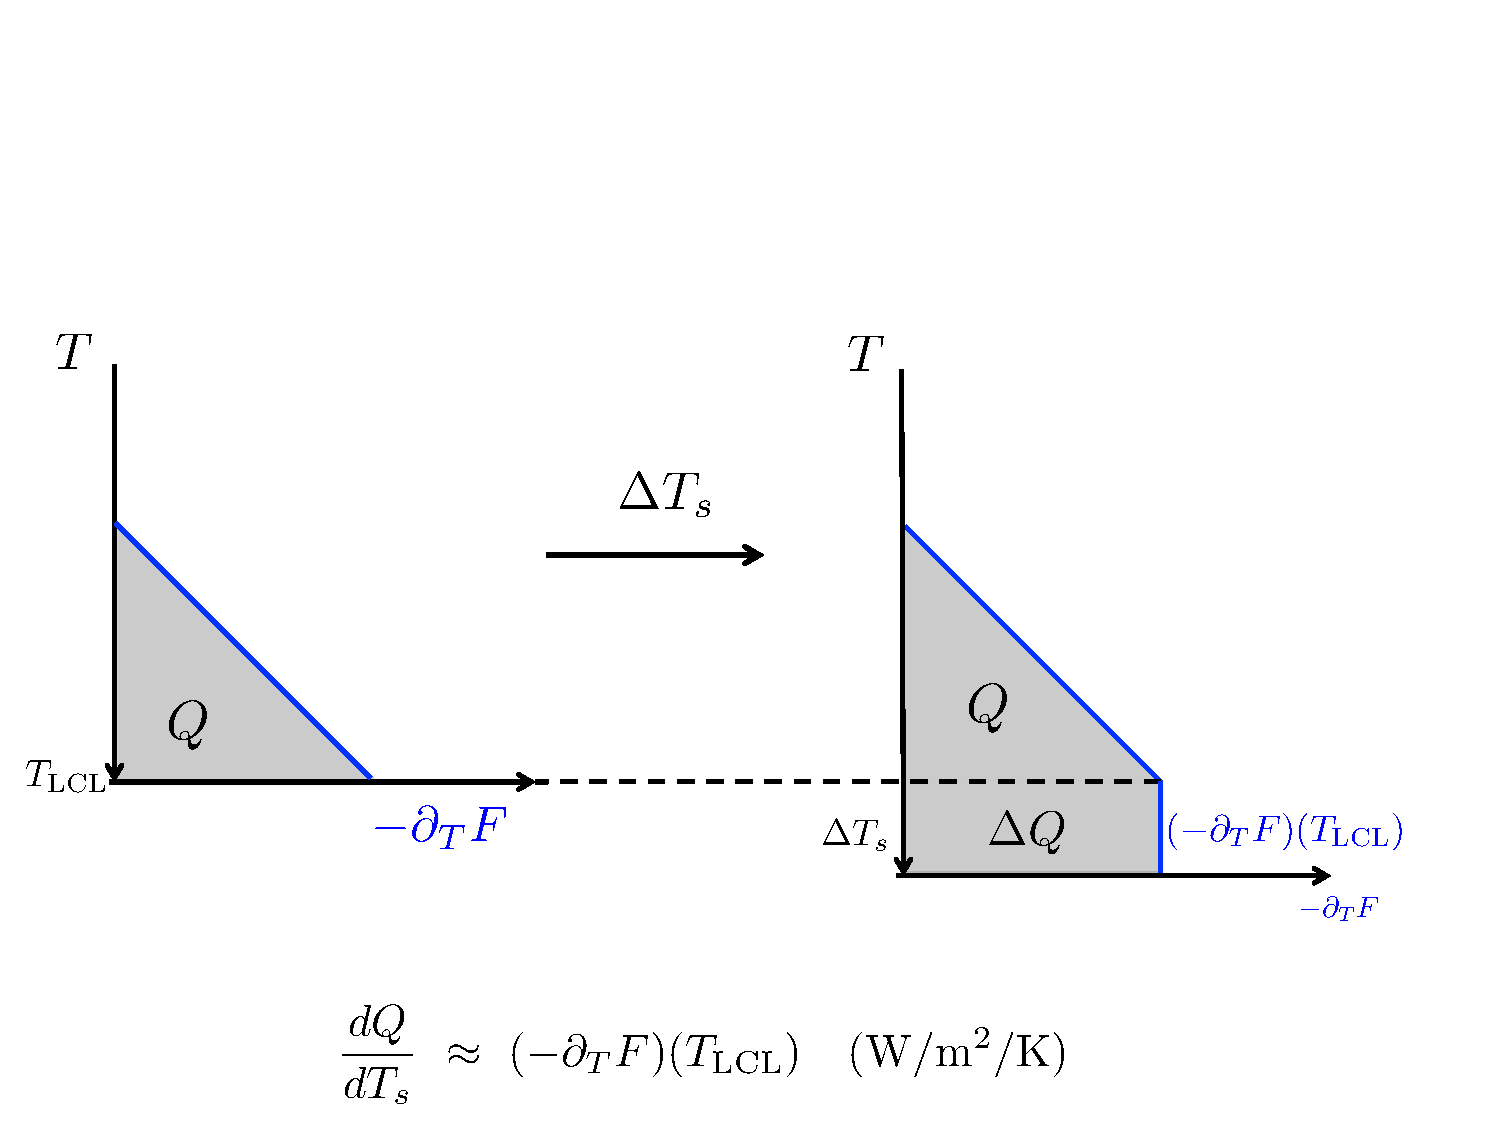
\includegraphics[scale=0.65,trim=0cm 0cm 0cm 5cm,clip=true]{../figures/dqdts_cartoon.pdf}
		\caption{Cartoon depicting the increase in $Q$ with \Ts\ in Eqn. \eqnref{dqdts}. Increasing the temperature range of the troposphere  exposes more of the \Ts-invariant curve $(\ppt F)(T)$ (blue lines). The contribution  of this newly exposed region to column-integrated cooling is given by Eqn. \eqnref{dqdts}.
		\label{dqdts_cartoon}
		}
	\end{center}
\end{figure}


%Figure Qnet_varsst
\begin{figure}[h]
	\begin{center}
			\includegraphics[scale=0.6]{../figures/Qnet_varsst.pdf}
		\caption{Column-integrated cooling $Q$ vs. \Ts\ (black circles), along with slopes $d Q/d \Ts$ (red lines) as diagnosed from \eqnref{dqdts}. These are shown for the SW (left), LW (center) and Net (right) channels.  The black dashed lines connect the black circles and give a benchmark slope against which to compare the red lines. The `Net' panel also gives CRM-diagnosed precipitation values in blue stars. See text for discussion.
		\label{Qnet_varsst}
		}
	\end{center}
\end{figure}


\bibliographystyle{apa}
\bibliography{/Users/nadir/Dropbox/bibtex_mendeley/library}


\end{document}

